% !TEX spellcheck = en_US
% !TEX spellcheck = LaTeX
\documentclass[a4paper,10pt, english]{article}
\usepackage{%
	amsfonts,%
	amsmath,%	
	etex,%
	amssymb,%
	amsthm,%
	babel,%
	bbm,%
	%biblatex,%
	caption,%
	centernot,%
	color,%
	enumerate,%
	epsfig,%
	epstopdf,%
	geometry,%
	graphicx,%
	hyperref,%
	latexsym,%
	mathtools,%
	multicol,%
	pgf,%
	pgfplots,%
	pgfplotstable,%
	pgfpages,%
	proof,%
	psfrag,%
	subfigure,%	
	tikz,%
	ulem,%
	url%
}	

\usepackage[mathscr]{eucal}
\usepgflibrary{shapes}
\usetikzlibrary{%
  arrows,%
	backgrounds,%
	chains,%
	decorations.pathmorphing,% /pgf/decoration/random steps | erste Graphik
	decorations.text,%
	matrix,%
  	positioning,% wg. " of "
  	fit,%
	patterns,%
  	petri,%
	plotmarks,%
  	scopes,%
	shadows,%
  	shapes.misc,% wg. rounded rectangle
  	shapes.arrows,%
	shapes.callouts,%
  	shapes%
}

\theoremstyle{plain}
\newtheorem{thm}{Theorem}[section]
\newtheorem{lem}[thm]{Lemma}
\newtheorem{prop}[thm]{Proposition}
\newtheorem{cor}[thm]{Corollary}

\theoremstyle{definition}
\newtheorem{defn}[thm]{Definition}
\newtheorem{conj}[thm]{Conjecture}
\newtheorem{exmp}[thm]{Example}
\newtheorem{assum}[thm]{Assumptions}
\newtheorem{axiom}[thm]{Axiom}

\theoremstyle{remark}
\newtheorem{rem}{Remark}
\newtheorem{note}{Note}

\newcommand{\norm}[1]{\left\lVert#1\right\rVert}
\newcommand{\indep}{\!\perp\!\!\!\perp}
\DeclarePairedDelimiter\abs{\lvert}{\rvert}%
%\DeclarePairedDelimiter\norm{\lVert}{\rVert}%
\newcommand{\tr}{\operatorname{tr}}
\newcommand{\R}{\mathbb{R}}
\newcommand{\Q}{\mathbb{Q}}
\newcommand{\N}{\mathbb{N}}
\newcommand{\E}{\mathbb{E}}
\newcommand{\Z}{\mathbb{Z}}
\newcommand{\B}{\mathscr{B}}
\newcommand{\C}{\mathcal{C}}
\newcommand{\T}{\mathscr{T}}
\newcommand{\F}{\mathcal{F}}
\newcommand{\G}{\mathcal{G}}
%\newcommand{\ba}{\begin{align*}}
%\newcommand{\ea}{\end{align*}}

\makeatletter
\def\th@plain{%
  \thm@notefont{}% same as heading font
  \itshape % body font
}
\def\th@definition{%
  \thm@notefont{}% same as heading font
  \normalfont % body font
}
\makeatother
\date{}
\title{Lecture 05: Renewal Theory}
\author{}

\begin{document}
\maketitle

\section{Renewal Theory}
One of the characterization for the Poisson process is of it being a counting process with \emph{iid} exponential inter-arrival times. Now we shall relax the ``exponential" part. 
\begin{defn} A counting process ${N(t),t \geq 0}$ with \emph{iid} general inter-arrival times is called a \textbf{renewal process}.
\end{defn}
As a result, we no longer have the nice properties such as Independent and stationary increments that Poisson processes had. However, we can still get some great results which also apply to Poisson Processes. 

\begin{defn}[Inter-arrival Times] Let $\{X_i: i \in \N\}$ be a sequence of non-negative \emph{iid} random variables with a common distribution $F$, with 
	\begin{enumerate}
		%\item Positive inter-arrival time,% i.e. $X_n \geq 0$,
		\item finite mean $\mu$, %i.e. $(0 \leq \mu = E[X_1] < \infty)$, and
		\item $F(0) < 1$.%= \Pr\{X_n \leq 0\} = \Pr\{X_n = 0\} < 1$.
	\end{enumerate}
\end{defn}
Second condition implies non-degenerate renewal process, if $F(0) = 1$ then it is a trivial process. We interpret $X_n$ as the time between $(n - 1)^{\text{st}}$ and the $n^{\text{th}}$ renewal event. 
\begin{defn}[Renewal Instants] Let $S_n$ denote the time of $n^{\text{th}}$ renewal, and assume $S_0 = 0$. Then, we have
\begin{align*} 
S_n = \sum_{i=1}^n X_i, \quad n\in \N. 
\end{align*}
\end{defn}
\begin{defn}[Renewal process] Let $\{N(t), t \geq 0\}$ be the counting process that counts number of events by time $t$. Then,
	\begin{align*} 
	N(t) = \sup\{n \in \N_0 : S_n \leq t\} = \sum_{n \in \N}1_{\{S_n \leq t\}}.
	\end{align*} 
	This counting process $\{N(t), t \geq 0\}$ is called a renewal process.
\end{defn}
\begin{lem}[Inverse Relationship]
	There is an inverse relationship between time of $n^{\text{th}}$ event $S_n$, and the counting process $N(t)$. That is
	\begin{align}
	\label{eq:InverseRelationship}
	\{S_n \leq t\} \iff \{N(t) \geq n\}.
	\end{align}
	%since $N(t) = \sum_{n \in \N}1_{\{S_n \leq t\}}$.
\end{lem}

\begin{lem}[Finiteness of $N(t)$]
	We are interested in knowing how many renewals occur per unit time. From SLLN, we have 
	\begin{align*} 
	\frac{S_n}{n} \to \mu \quad \mbox{a.s.}
	\end{align*} 
	Since $\mu > 0$, we must have $S_n$ growing arbitrarily large as $n$ increases. Thus,
	$S_n$ can be finite for at most finitely many $n$. Therefore, $N(t)$ must be finite,
	and
	\begin{align*} 
	N(t) = \max\{n \in \N_0 : S_n \leq t\}.
	\end{align*} 
\end{lem}

\subsection{Distribution of N(t)}
We need to know the distribution of $N(t)$. 
\begin{lem} Counting process $N(t)$ assumes non-negative integer values with distribution
	\begin{align*}
	\Pr\{N(t) = n\} = \Pr\{S_n \leq t\} - \Pr\{S_{n+1} \leq t\} = F_n(t) - F_{n+1}(t).
	\end{align*}
\end{lem}
\begin{proof} It follows from~\eqref{eq:InverseRelationship}.
\end{proof}
\begin{defn} Let $F_n$ be the distribution of renewal instant $S_n$ i.e. $\Pr\{S_n \leq t\} = F_n(t)$.
\end{defn}
\begin{lem} Distribution $F_n$ of renewal instant $S_n$  is given inductively by
	\begin{xalignat*}{3}
		&F_1 = F,&&F_n = F_{n-1}\ast F,
	\end{xalignat*}
	where $\ast$ denotes convolution.
\end{lem}
\begin{proof} It follows from induction over sum of \emph{iid} random variables.
\end{proof}
%Denote $F_n = F^{*(n)}$ where $*$ denotes convolution. Essentially, $F^{*(n)}$ is the distribution of $S_n$.
\begin{defn} We define $m(t) = \mathbb{E}[N(t)]$ to be the \textbf{renewal function}.
\end{defn}
We are interested in the following two quantities.
\begin{xalignat*}{3}
	&m(t) = \mathbb{E}[N(t)].
	%, &&M_{N(t)}(\theta) = \E[e^{\theta N(t)}].
\end{xalignat*}

\begin{prop} Renewal function can be expressed in terms of distribution of renewal instants as
	\begin{align*} 
	m(t) = \sum_{n \in \N} F_n(t).
	\end{align*}
\end{prop}
\begin{proof} It follows from~\eqref{eq:InverseRelationship} and definitions,
	\begin{align*}
	m(t) &= \mathbb{E}[N(t)] \\ &= \sum_{n \in \N} \Pr\{N(t) \geq n\} (\because expectation~can~be~defined~ in~ terms~ of~ \emph{ccdf}) \\ &= \sum_{n \in \N} \Pr\{S_n \leq t\} = \sum_{n \in \N} F_n(t)
	\end{align*}
	\\
	Alternatively,
	\begin{align*}
	m(t) &= \mathbb{E}[N(t)] \\
	&= \mathbb{E} \left[\sum_{n \in \N} \mathbb{I}_{\{S_n \leq t\}} \right] \\
	&= \sum_{n \in \N} \mathbb{E} \left[ \mathbb{I}_{\{S_n \leq t\}} \right] (\because Monotone~ Convergence~ Theorem) \\
	&= \sum_{n \in \N} \Pr\{S_n \leq t\} = \sum_{n \in \N} F_n(t)
	\end{align*}
\end{proof}

\begin{prop} Renewal function is bounded for all finite times.
	%\begin{align*} 
	%m(t) < \infty \quad \forall 0 \leq t < \infty
	%\end{align*}
\end{prop}
\begin{proof}
	Since we assumed that $\Pr\{X_n = 0\} < 1$, it follow from continuity of probabilities that there exists $\alpha > 0$, such that $\Pr\{X_n \geq \alpha\} >0$. Define
	\begin{align*}
	\bar{X}_n = \alpha 1_{\{X_n \geq \alpha\}}.
	\end{align*}
	Let $\bar{N}(t)$ denote the renewal process with inter-arrival times $\bar{X}_n$. Note that since $X_i$'s are \emph{iid}, so are $\bar{X}_i$ (which will be evident from the proof of the distribution function of the number of arrivals till time t). In fact, the arrivals now happen at multiples of $\alpha$. And yes, they stack. Moreover, $X_n \geq \bar{X}_n$. \\
	
	\begin{align*}
	Pr\{Number ~of ~arrivals ~at ~time ~0 ~= n\} &= Pr\{\bar{X_1}=\bar{X_2}=\ldots=\bar{X_n}=0,\bar{X_{n+1}}=\alpha\} \\
	&= Pr\{X_1 < \alpha,X_2 < \alpha,\ldots,X_n < \alpha,X_{n+1} \geq \alpha\} \\
	&= \prod_{i=1}^{n} Pr\{X_i < \alpha\} . Pr\{X_{n+1} \geq \alpha \} ~(\because ~of ~independence) \\
	&= \left(1- Pr\{X_1 \geq \alpha \}\right) ^{n} . Pr\{X_1 \geq \alpha\}~(\because ~of ~identicality) 
	\end{align*}
	
	The number of arrivals till time $t$ therefore is Geometric with mean $\frac{1}{P[X_n \geq \alpha]}$. Thus 
	\begin{align*}
	E[\bar{N}(t)] = \frac{\lfloor\frac{t}{\alpha} \rceil + 1}{P[X_n \geq \alpha]} \leq \frac{\frac{t}{\alpha} \rceil + 1}{P[X_n \geq \alpha]} < \infty
	\end{align*}
	Since $E[N(t)] \leq E[\bar{N}(t)]$ which follows from $N(t) \leq \bar{N}(t)$, we are done.
\end{proof} 
\section{Limit Theorems}

\begin{lem}
	Let $N(\infty) := \lim_{t \to \infty} N(t)$. Then, it is easy to see that $\Pr\{N(\infty) = \infty\} = 1$.	
\end{lem}

\begin{proof}
	It suffices to show $\Pr\{N(\infty) < \infty\} = 0$. We have
	\begin{flalign*}
	\Pr\{N(\infty) < \infty\} &= \Pr\{\bigcup_{n \in \N} \{N(\infty) < n\}\}\\
	&= \Pr\{\bigcup_{n \in \N} \{S_n = \infty\}\} = \Pr\{\bigcup_{n \in \N} \{X_n = \infty\}\} \\
	&\leq \sum_{n \in \N}\Pr\{X_n = \infty\} =0.
	\end{flalign*}
	The last step follows from the fact that $E[X_n] < \infty$.
\end{proof}
\begin{thm}[Basic Renewal Theorem]
	
	
	\begin{align*}
	\lim_{t \to \infty} \frac{N(t)}{t} = \frac{1}{\mu} \quad \mbox{almost surely}.
	\end{align*}
\end{thm}
[
Notice that $N(t)$ increases to infinity with time. We are interested in rate of increase of $N(t)$ with $t$. Note that $S_{N(t)}$ represents the time of last renewal before $t$, and $S_{N(t)+1}$ represents the time of first renewal after time $t$. ] \\

\begin{proof}
	% Need picture here
	%0 ------- S_{N(t)}---t ---- S_{N(t)+1} ------------
	\begin{figure}
		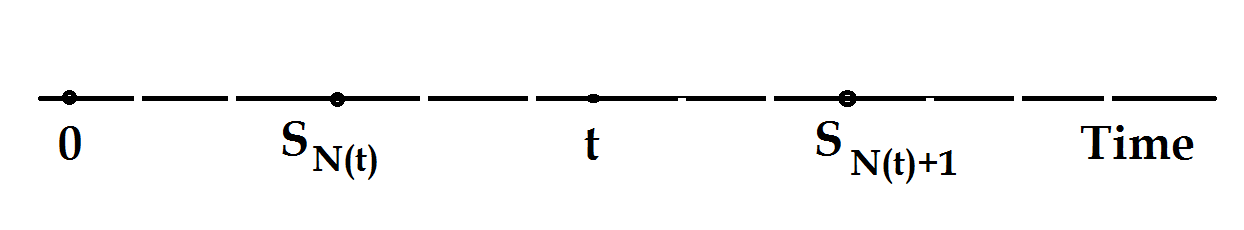
\includegraphics[width=\linewidth]{Figures/lecture_5_fig_1.png}
	\end{figure}
	Consider $S_{N(t)}$. By definition, we have
	\[S_{N(t)} \leq t < S_{N(t)+1}\]
	Dividing by $N(t)$, we get 
	\[\frac{S_{N(t)}}{N(t)} \leq \frac{t}{N(t)} < \frac{S_{N(t)+1}}{N(t)}\]
	By Strong Law of Large Numbers (SLLN) and the previous result, we have
	\[\lim_{t \to \infty}\frac{S_{N(t)}}{N(t)} = \mu \quad \mbox{a.s.}\] 
	Also
	\[\lim_{t \to \infty} \frac{S_{N(t)+1}}{N(t)} = \lim_{t \to \infty} \frac{S_{N(t)+1}}{N(t)+1}.\frac{N(t)+1}{N(t)} \]
	Hence by Squeeze Theorem, the result follows.
\end{proof}


\subsubsection{Example}
Suppose, you are in a casino with infinitely many games. Every game has a probability of win $X$, \emph{iid} uniformly distributed between $(0,1)$. One can continue to play a game or switch to another one. We are interested in a strategy that maximizes the long-run proportion of wins.

Let $N(n)$ denote the number of losses in $n$ plays. Then fraction of wins $P_W(n)$ is given by 
\begin{align*}
P_W(n) = \frac{n-N(n)}{n}.
\end{align*}
We pick a strategy where any game is selected to play, and continue to be played till the first loss. Note that, time till first loss is geometrically distributed with mean $\frac{1}{1-X}$. We shall show that this fraction approaches unity as $n \to \infty$. By the previous proposition, we have:
\begin{align*}
\lim_{n \to \infty} \frac{N(n)}{n} &= \frac{1}{E[\mbox{Time till first loss}]} \\
&= \frac{1}{E\left[\frac{1}{1-X}\right]} = \frac{1}{\infty} = 0
\end{align*}
Hence Renewal theorems can be used to compute these long term averages. We'll have many such theorems in the following sections.

\subsection{Wald's Lemma}
Before we get into Wald's Lemma, let us first define what a stopping time is.
\begin{defn}[Stopping Time]
	Let $\{X_n: n\in \N\}$ be independent random variables. Then $T$, an integer random variable, is called a stopping time wrt this sequence if $\{N=n\}$ depends only on $\{X_1,\cdots,X_n\}$ and is independent of $X_{n+1}, X_{n+2},\cdots$. 
\end{defn}
Intuitively, if we observe the $X_n$'s in sequential order and $N$ denotes the number observed before stopping then. Then, we have stopped after observing, $X_1, \ldots, X_N$, and before observing $X_{N+1}, X_{N+2}, \ldots$. 
The intuition behind a stopping time is that it's value is determined by past and present events but NOT by future events. 
\begin{exmp}
	For instance, while traveling on the bus, the random variable measuring ``Time until bus crosses Majestic and after that one stop" is a stopping time as it's value is determined by events before it happens. On the other hand ``Time until bus stops before Majestic is reached'' would not be a stopping time  in the same context. This is because we have to cross this time, reach Majestic and then realise we have crossed that point. 
\end{exmp}
\begin{exmp} Consider $X_n \in \{0,1\}$ \emph{iid} Bernoulli$(1/2)$. Then $N = min \{n \in \N:\quad \sum_{i=1}^n X_i = 1\}$ is a stopping time. For instance, $Pr\{N=2\} = Pr\{X_1=0,X_2=1\}$ and hence $ N $ is a stopping time by definition.
\end{exmp}
\begin{exmp}[Random Walk Stopping Time] Consider $X_n$ \emph{iid} bivariate random variables with 
	\begin{align*}
	\Pr\{X_n = 1\} = \Pr\{X_n = -1\} = \frac{1}{2}. 
	\end{align*}
	Then $N = min \{n \in \N:\quad \sum_{i=1}^n X_i = 1\}$ is a stopping time.
\end{exmp}

\emph{Properties}: Let $N_1,N_2$ be two stopping times wrt $\{X_i : i \in \N \} $ then,
\begin{itemize}
	\item $N_1+N_2$ is a stopping time.
	\item $\min \{N_1,N_2\} $ is a stopping time.
\end{itemize}
\begin{proof}
\begin{itemize}
	\item 
	\begin{align*}
	\{N_1+N_2 \leq n\} &= \bigcup_{i=0}^{n} \{N_1+N_2 = i\}
	\\
	&= \bigcup_{i=0}^{n} \bigcup_{k=0}^{i} \{N_1 = k\} \cap \{N_2 = i-k\}
	\\
	& \!\perp\!\!\!\perp \{X_{n+1},X_{n+2},\ldots\}
	\end{align*}
	Hence, $N_1+N_2$ is a stopping time.
	\item 
	\begin{align*}
	\{\min \{N_1,N_2\} > n\} = \{N_1 > n\} \cap \{N_2 > n\}
	\\
	\implies \{\min \{N_1,N_2\} \leq n\} &= \{N_1 \leq n\} \cap \{N_2 \leq n\}
	\\
	& \!\perp\!\!\!\perp \{X_{n+1},X_{n+2},\ldots\}
	\end{align*}
	Hence, $\min \{N_1,N_2\} $ is a stopping time.
\end{itemize}
\end{proof}

\begin{lem}[Wald's Lemma]
	Let $\{X_i:\quad i\in \N\}$ be \emph{iid} random variables with finite mean $E[X_1]$ and let $N$ be a stopping time with respect to this set of variables, such that $E[N] < \infty$. Then
	\[E\left[\sum_{n=1}^N X_n\right] = E[X_1]E[N]\]
\end{lem}
\begin{proof}
	\begin{align}
	E\left[\sum_{n=1}^N X_n\right] &= E\left[\sum_{n \in \N} X_n 1_{\{N \geq n\}}\right]  \\
	&= \sum_{n \in \N} E\left[X_n 1_{\{N \geq n\}}\right] \label{tricky}
	\end{align}
	I'd like to point out here that in step (\ref{tricky}), you cannot always exchange infinite sums and expectations. But here you can do so, because of the application of Monotone Convergence Theorem. Refer Ross/Wolff for more information. Regardless, to proceed, we need to show that $N \geq n$ is independent of $X_k, \quad k \geq n$. To this end, observe that 
	\begin{align*}
	\{N \geq k\} = \{N < k\}^c = \{N \leq k-1\}^c = \left(\bigcup_{i=1}^{k-1} \{N = i\}\right)^c. 
	\end{align*}
	Since, $N$ is a stopping time and by definition $\{N=i\}$ depends only on $\{X_1,\ldots, X_i\}$. Therefore, $\{N \geq k\}$ depends only on $\{X_1,\ldots, X_{k-1}\}$, and is independent of the future and present samples. Therefore, we can write
	\begin{align*}
	\sum_{n \in \N} E\left[X_n 1_{\{N \geq n\}}\right] &= \sum_{n \in \N} E\left[X_n\right]E\left[ 1_{\{N \geq n\}}\right] \\
	&= E\left[X_1\right] \sum_{n \in \N} \Pr\{N \geq n\} \\
	&= E[X_1]E[N] ~(\because expectation~can~be~defined~ in~ terms~ of~ \emph{ccdf}).
	\end{align*} 
\end{proof}

\begin{prop}[Wald's Lemma for Renewal Process] \label{prop:WaldRenewal}
	Let $\{X_n, n \in \N\}$ be \emph{iid} inter-arrival times of a renewal process $N(t)$ with $E[X_1] < \infty$, and let $m(t) = E[N(t)]$ be its renewal function. Then, $N(t)+1$ is a stopping time and 
	\begin{align*}
	E\left[\sum_{i=1}^{N(t)+1}X_i\right] = E[X_1][1+m(t)]
	\end{align*}
\end{prop}
\begin{proof} It is easy to see that $\{N(t)+1=n\}$ depends solely on $\{X_1,\ldots,X_n\}$ from the discussion below.
	\begin{align*}
	\left\{N(t) + 1 = n \right\} \iff \{S_{n-1} \leq t < S_n\} \iff \left\{\sum_{i=1}^{n-1} X_i \leq t < \sum_{i=1}^{n-1} X_i + X_n\right\}
	\end{align*}
	Thus $N(t)+1$ is a stopping time, and the result follows from Wald's Lemma.
\end{proof}

\subsection{Elementary Renewal Theorem}
Basic renewal theorem implies $N(t)/t$ converges to $1/\mu$ almost surely. Now, we are interested in convergence of $E[N(t)]/t$. Note that this is not obvious, since almost sure convergence doesn't imply convergence in mean. Consider the following example.
\begin{exmp}
	\begin{align*}
	Y_n = \begin{cases}
	n, & \mbox{ w.p.  } 1/n,\\
	0, & \mbox{ w.p.  } 1- 1/n.
	\end{cases}
	\end{align*}
	Then, $\Pr\{ Y_n = 0 \} = 1 - 1/n$. %Then $\sum \Pr\{Y_n > \epsilon\} < \infty$. Hence by Borel Cantelli Lemma, $Y_n \to 0$
	That is $Y_n \to 0$ a.s. However, $E[Y_n] = 1$ for all $n \in \N$. So $E[Y_n] \to 1$.
\end{exmp}
Even though, basic renewal theorem does \textbf{NOT} imply it, we still have $E[N(t)]/t$ converging to $1/\mu$.

\begin{thm}[Elementary Renewal Theorem] Let $m(t)$ denote mean $E[N(t)]$ of renewal process $N(t)$, then under the hypotheses of basic renewal theorem, we have 
	\begin{align*}
	\lim_{t \to \infty}\frac{m(t)}{t} = \frac{1}{\mu}.
	\end{align*}
\end{thm}
\begin{proof}
	Take $\mu < \infty$. We know that $S_{N(t)+1} > t$. Therefore, taking expectations on both sides and using Proposition~\ref{prop:WaldRenewal}, we have 
	\begin{align*}
	\mu (m(t) + 1) > t.
	\end{align*}
	Dividing both sides by $\mu t$ and taking $\liminf$ on both sides, we get
	\begin{align}
	\label{eq:LiminfMean}
	\liminf_{t \to \infty} \frac{m(t)}{t} \geq \frac{1}{\mu}.
	\end{align}
	
	%Thus we now have to show 
	%\[\limsup_{t \to \infty} \frac{m(t)}{t} \leq \frac{1}{\mu}\]
	We employ a truncated random variable argument to show the reverse inequality. We define truncated inter-arrival times $\{\bar{X}_n\}$ as 
	\begin{align*}
	\bar{X}_n = X_n 1_{\{X_n \leq M\}} + M1_{\{X_n > M\}}.
	\end{align*}
	We will call $E[\bar{X}_n] = \mu_M$. Further, we can define arrival instants $\{\bar{S}_n\}$ and renewal process $\bar{N}(t)$ for this set of truncated inter-arrival times $\{\bar{X}_n\}$ as 
	\begin{align*}
	\bar{S}_n &= \sum_{k=1}^n \bar{X}_k, & \bar{N}(t) &= \sup\{n \in \N_0: \bar{S}_n \leq t\}.
	\end{align*}
	Note that since $S_n \geq \bar{S}_n$, number of arrivals would be higher for renewal process with truncated random variables, i.e. 
	\begin{align}
	\label{eq:TruncRenewalInequality}
	N(t) \leq \bar{N}(t).
	\end{align}
	Further, due to truncation of inter-arrival time, next renewal happens with-in $M$ units of time, i.e.
	\begin{align*}
	\bar{S}_{N(t)+1} \leq t+M.
	\end{align*}
	Taking expectations on both sides in the above align, using Proposition~\ref{prop:WaldRenewal}, dividing both sides by $t \mu_M$ and taking $\limsup$ on both sides, we obtain
	\begin{align*}
	\limsup_{t \to \infty}\frac{\bar{m(t)}}{t} \leq \frac{1}{\mu_M}.
	\end{align*}
	Taking expectations on both sides of~\eqref{eq:TruncRenewalInequality} and letting $M$ go arbitrary large on RHS, we get
	\begin{align}
	\label{eq:LimsupMean}
	\limsup_{t \to \infty}\frac{m(t)}{t} \leq \frac{1}{\mu}.
	\end{align}
	%Now observe that LHS is independent of $M$. Take limits $M \to \infty$, noting that $\mu_M \to \mu$ (Why?) to get
	%\[\limsup_{t \to \infty}\frac{m(t)}{t} \leq \frac{1}{\mu}\]
	%Putting it all together,
	%\[\lim_{t \to \infty}\frac{m(t)}{t} = \frac{1}{\mu}\]
	Result for finite $\mu$ follows from~\eqref{eq:LiminfMean} and~\eqref{eq:LiminfMean}. When $\mu$ grows arbitrary large, results follow from~\eqref{eq:LiminfMean}, where RHS is zero. 
\end{proof}

\subsection{Central Limit for Renewal Processes}
\begin{thm}
Let $X_n$ be \emph{iid} random variables with $\mu = E[X_n] < \infty$ and $\sigma^2 = Var(X_n) < \infty$. Then
\[\frac{N(t)-\frac{t}{\mu}}{\sigma \sqrt{\frac{t}{\mu^3}}} \to^d N(0,1) \]
\end{thm}
\begin{proof}
Take $u = \frac{t}{\mu} + y \sigma \sqrt{\frac{t}{\mu^3}}$. We shall treat $u$ as an integer and proceed, the proof for general $u$ is an exercise. Recall that $\{N(t) < u\} \iff \{S_u > t\}$. By equating probability measures on both sides, we get
\begin{align*}
\Pr\{N(t) < u\} = \Pr\left\{\frac{S_u - u\mu}{\sigma \sqrt{u}} > \frac{t - u\mu}{\sigma \sqrt{u}}\right\} = \Pr\left\{\frac{S_u - u\mu}{\sigma \sqrt{u}} > -y\left(1 + \frac{y\sigma}{\sqrt{tu}}\right)^2\right\}.
\end{align*}
By central limit theorem, $\frac{S_u - u\mu}{\sigma \sqrt{u}}$ converges to a normal random variable with zero mean and unit variance as $t$ grows. Also, note that 
\begin{align*}
\lim_{t \to \infty} -y\left(1 + \frac{y\sigma}{\sqrt{tu}}\right)^2 = -y.
\end{align*}
These results combine with the symmetry of normal random variable to give us the result.
\end{proof}
\end{document}